%!TEX TX-program = xelatex
%
%%%%%%%%%%%%%%%%%%%%
%
% Title: 10 220511 向量
% Author: Eason S.
% Date: 220511
% Institude: Shanghai Experimental School
% Email: eason.syc@icloud.com
% GitHub: https://github.com/EasonSYC
% GitHub Repository: https://github.com/EasonSYC/Maths_Error
%
%%%%%%%%%%%%%%%%%%%%

\documentclass[8pt]{article}
\usepackage{allan-eason}

\usetikzlibrary{positioning}
\usetikzlibrary{svg.path}

\graphicspath{ {./images/} }

\newcommand{\Date}{220511}
\newcommand{\Test}{向量}

\newcommand{\Author}{Eason S.}
\newcommand{\Title}{\textcolor{allandarkblue}{\Date}\ \textcolor{allancyan}{\Test}\ 题目选解}

\author{\Author}
\title{\Title}
\date{}

\geometry{a4paper, scale=0.8}

\lhead{\Title}

\begin{document}

	\maketitle

	\tableofcontents

	\section{填空题}
		\begin{easonproblem}
			设\(\vec{a}\)与单位向量\(\vec{b}\)的数量积为\(-2\), 则\(\vec{a}\)在\(\vec{b}\)方向上的数量投影为?.
			\subproblem
			\answord{\(-2\).} 利用\(\displaystyle \Prj{\vec{b}}{\vec{a}} = \vec{a} \cos \ang{\vec{a}, \vec{b}} = \frac{\vec{a} \cdot \vec{b}}{\abs{\vec{b}}}\) (向量的数量积与向量的数量投影之间的联系) \cite{linearalgebra-tj}.
		\end{easonproblem}

		\begin{easonproblem}
			平面直角坐标系中\(O\)为坐标原点, \(M(3, 4), B(3, 1), \ray{AC} = (-1, 1)\), 且\(\ray{OM}\)为\(\ray{AB}\)的位置向量, 则点\(C\)的坐标为?.
			\subproblem
			\answord{\((-1, -2)\).} 向量的坐标表示.
		\end{easonproblem}

		\begin{easonproblem}
			与非零向量\(\vec{a} = (m, n)\)垂直且模长为\(2\)的向量可表示为? (用坐标表示).
			\subproblem
			\answord{\(\displaystyle \left(\pm \frac{2n}{\sqrt{m^2 + n^2}}, \mp \frac{2m}{\sqrt{m^2 + n^2}}\right) = \left(\pm \frac{2n\sqrt{m^2 + n^2}}{m^2 + n^2}, \mp \frac{2m\sqrt{m^2 + n^2}}{m^2 + n^2}\right)\).} 向量的坐标表示下的内积; 向量的内积的取值范围与向量之间位置关系的联系.
		\end{easonproblem}

		\begin{easonproblem}
			\(\frac{x_1}{y_1} + \frac{y_2}{x_2} = 0\)是\(\left(x_1 \vec{i} + y_1 \vec{j}\right)\perp \left(x_2 \vec{i} + y_2 \vec{j}\right)\)的?条件. \athword{作者认为此处应该补充条件: \(\vec{i}, \vec{j}\)为\(\RR^2\)上的一个标准正交基 更为合适.} \cite{owenxuanswer}
			\subproblem
			\answord{充分非必要.} 向量的内积的取值范围与向量之间位置关系的联系; 向量的内积对向量的线性组合的分配律. 
		\end{easonproblem}

		\begin{easonproblem}
			设\(\abs{\vec{a}} = 3, \abs{\vec{a} - \vec{b}} = 9,\)则\(\abs{\vec{b}}\)的取值范围为?.
			\subproblem
			\answord{\([5, 11]\).} 向量的三角不等式 \(\abs{\abs{\vec{a}} - \abs{\vec{b}}} \leq \abs{\vec{a} \pm \vec{b}} \leq \abs{\abs{\vec{a}} + \abs{\vec{b}}}\).
		\end{easonproblem}

		\begin{easonproblem}
			\(\vec{a} = (3m-2, 1), \vec{b} = (m^2+1, 2)\), 若\(9\vec{a} + 3\vec{b}\)与\(\vec{a} - \vec{b}\)共线, 则实数\(m\)的值为?.
			\subproblem
			\answord{\(1 \lgor 5\).} 向量的坐标表示下的共线.
		\end{easonproblem}

		\begin{easonproblem}
			已知\(A, B, C\)坐标依次为\((1, 2), (2, 3), (5, 10)\), 则\(\triangle ABC\)的面积为?.
			\subproblem
			\answord{\(2\).} 行列式视角下的三角形面积公式. \cite{detarea}
			\begin{align*}
				S_{\triangle ABC} &= \frac{1}{2} \abs{\abs{
									\begin{array}{ccc}
										x_1 & x_2 & x_3\\
										y_1 & y_2 & y_3\\
										1   & 1   & 1  
									\end{array}
								}}\\
				                  &= \frac{1}{2} \abs{\abs{
									\begin{array}{ccc}
										1 & 2 & 5\\
										2 & 3 & 10\\
										1 & 1 & 1  
									\end{array}
								}}\\
								  &\xlongequal{c_3-2c_1} \frac{1}{2} \abs{\abs{
									\begin{array}{ccc}
										1 & 2 & 0\\
										2 & 3 & 0\\
										1 & 1 & -4  
									\end{array}
								}}\\
								  &\xlongequal[\text{按}c_3\text{展开}]{c_3\div (-4)} \frac{1}{2} \abs{(-4) \abs{
									\begin{array}{cc}
										1 & 2\\
										2 & 3\\ 
									\end{array}
								}}\\
								&= 2.
 			\end{align*}
		\end{easonproblem}

		\begin{easonproblem}
			如图, 正方形\(ABCD\)的边长为\(1\), \(E\)为边\(BC\)的中点, \(F\)为边\(CD\)上一点, 若\(\ray{AE} \cdot \ray{AF} = \ray{AE}^2\), 则\(\abs {\ray{AF}}\)为?.
			
			\[	
			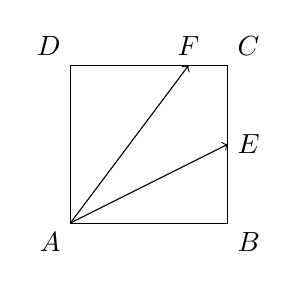
\begin{tikzpicture}[scale = 2]
				\draw[black] (0, 0)--(0, 1)--(1, 1)--(1, 0)--(0, 0) node at (0, 0) [anchor = north east] {\(A\)} node at (1, 0) [anchor = north west] {\(B\)} node at (1, 1) [anchor = south west] {\(C\)} node at (0, 1) [anchor = south east] {\(D\)};
				\draw[black, ->] (0, 0)--(1, 0.5) node at (1, 0.5) [anchor = west] {\(E\)};
				\draw[black, ->] (0, 0)--(0.75, 1) node at (0.75, 1) [anchor = south] {\(F\)};
			\end{tikzpicture}
			\]

			\subproblem
			\answord{\(\frac{5}{4}\).} 向量的内积对向量的线性组合的分配律; 向量的内积的取值范围与向量之间位置关系的联系; 一线三等角.
		\end{easonproblem}

		\begin{easonbigproblem}
			如图, \(A, B, C, D\)四点共线, \(P, Q\)为直线外两点, 已知\(AB:BC=2:3, \ray{PB} = \frac{3}{2} \ray{PC} - \frac{1}{2} \ray{PD}\), 若\(\ray{QB} = \lambda \ray{QA} + \mu \ray{QD}\), 则\(\lambda - \mu\)的值为?.

			\[	
				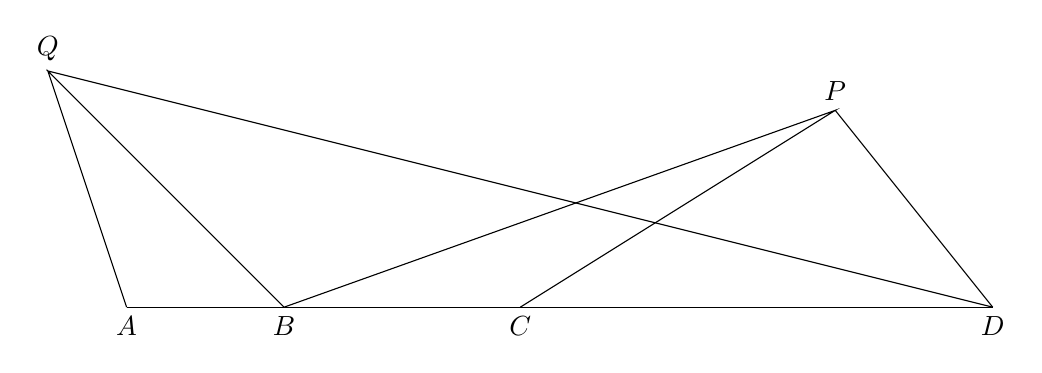
\begin{tikzpicture}
					\draw[black] (0, 0)--(2, 0)--(5, 0)--(11, 0) node at (0, 0) [anchor = north] {\(A\)} node at (2, 0) [anchor = north] {\(B\)} node at (5, 0) [anchor = north] {\(C\)} node at (11, 0) [anchor = north] {\(D\)};
					\draw[black] (0, 0)--(-1, 3)--(2, 0)--(-1, 3)--(11, 0) node at (-1, 3) [anchor = south] {\(Q\)};
					\draw[black] (2, 0)--(9, 2.5)--(5, 0)--(9, 2.5)--(11, 0) node at (9, 2.5) [anchor = south] {\(P\)};
				\end{tikzpicture}
			\]

			\subbigproblem
			\answord{\(\displaystyle \frac{7}{11}\).} 向量的线性组合.

			\begin{align*}
				\ray{PB} = \frac{3}{2} \ray{PC} - \frac{1}{2} \ray{PD} = \ray{PC} + \ray{CB} &\Rightarrow \frac{1}{2} \ray{PC} = \ray{CB} + \frac{1}{2} \ray{PD}\\
				&\Rightarrow \ray{PC} = \ray{PD} + 2 \ray{CB}\\
				&\Rightarrow \ray{DC} = 2\ray{CB}\\
				&\Rightarrow AB:BC:CD = 2:3:6.
			\end{align*}

			\begin{align*}
				\ray{QB} &= \ray{QA} + \ray{AB}\\
				         &= \lambda \ray{QA} + \mu \ray{QD}\\
						 &= \lambda \ray{QA} + \mu \left(\ray{QA} + \frac{11}{2} \ray{AB}\right)
			\end{align*}

			于是有

			\[
				\left\{
					\begin{array}{rcl}
						\lambda + \mu &=& 1,\\
						\frac{11}{2} \mu &=& 1,
					\end{array}
				\right.
				\Rightarrow
				\left\{
					\begin{array}{rcl}
						\lambda &=& \frac{9}{11},\\
						\mu &=& \frac{2}{11}.
					\end{array}
				\right.
			\]

		\end{easonbigproblem}

		\begin{easonbigproblem}
			以下命题中, 所有真命题的序号为?.
			\begin{enumerate}[label = \calword{(\arabic*)}]
				\item 若\(\vec{a}\)与\(\vec{b}\)可作为平面向量的一组基, 则\(\vec{a}, \vec{b} \neq \vec{0}\).
				\item 若\(\vec{a}\)和\(\vec{b}\)非共线, 则平面上任意向量\(\vec{c}\)关于\(2 \vec{a} + \vec{b}\)和\(\vec{a} + \vec{b}\)的分解均存在且唯一.
				\item 若\(\vec{a} \parallel \vec{b}\), 则\(\vec{a} + \vec{b} = \lambda \vec{a} + \mu \vec{b}\)的充要条件为\(\lambda = \mu = 1\).
				\item 若\(\vec{a} \parallel \vec{b}\), 且\(\vec{c}\)与\(\vec{a}, \vec{b}\)均不共线, 则\(\vec{c}\)关于\(\vec{a}\)与\(\vec{b}\)的分解不存在.
			\end{enumerate}
			\subbigproblem
			\answord{(1) (2) (4).} 向量的线性组合.
			\begin{enumerate}[label = \calword{(\arabic*)}]
				\item 在同构于\(\RR^n\)的向量空间 (即\(n\)维向量空间) 中的一组基\(A: \vect{a}_1, \vect{a}_2, \ldots, \vect{a}_n\)必然有\(\vect{a}_1, \vect{a}_2, \ldots, \vect{a}_n \neq \vect{0}\) (因为\(\mathrm{r}(\vect{A}) = n\)). 本题中, \(\vec{a}, \vec{b}\)为平面\(\RR^2\) (即\(2\)维向量空间) 上的一组基, 则必然有\(\mathrm{r} (\vect{a}, \vect{b}) = 2\), 有\(\vect{a}, \vect{b} \neq \vect{0}\). \cite{linearalgebra-tj}
				\item 显然有\((2\vect{a} + \vect{b}, \vect{a} + \vect{b}) \sim (\vect{a}, \vect{a} + \vect{b}) \sim (\vect{a}, \vect{b})\), 即向量组\(\vect{a}, \vect{b}\)与向量组\(2\vect{a} + \vect{b}, \vect{a} + \vect{b}\)等价. 同时有\(\mathrm{r} (\vect{a}, \vect{b}) = 2 = \mathrm{r}(2\vect{a} + \vect{b}, \vect{a} + \vect{b})\) (非共线, 线性无关), 则向量组\(2\vect{a} + \vect{b}, \vect{a} + \vect{b}\)是线性空间\(\RR^2\)上的一个基. \cite{linearalgebra-pearson}
    			\item 考虑\(\vec{a} = \vec{b} = \vec{0}\), 则\(\forall \lambda, \mu \in \RR: \vec{a} + \vec{b} = \lambda \vec{a} + \mu \vec{b} = \vec{0}\).
       			\item 假设\(\vect{c} = \lambda \vect{a} + \mu \vect{b}, \lambda, \mu \in \RR\), 由已知有\(\vect{a}, \vect{b}\)线性相关, 则必然有\(\vect{c} = \lambda \vect{a} + \mu \vect{b}\)可由\(\vect{a}, \vect{b}\)线性表示, 继而有\(\vect{a}, \vect{b}, \vect{c}\)线性相关, 与条件矛盾.
			\end{enumerate}
		\end{easonbigproblem}
	
	\newpage
	\section{解答题}
		
		\begin{easonproblem}
			设\(\vec{a} = (3, -4), \vec{b} = (2, -1)\),
			\begin{enumerate} [label = \calword{(\arabic*)}]
				\item 求\(\vec{a}\)与\(2\vec{b} - \vec{a}\)的夹角.
				\item 求\(\vec{a}\)在\(\left(2\vec{b} - \vec{a}\right)\)方向上的投影向量 (用坐标表示).
			\end{enumerate}
			\subproblem
			\answord{\(\displaystyle \pi - \arccos \left(\frac{\sqrt{5}}{5}\right)\); \((-1, -2)\).} 向量的投影. \cite{duckduckanswer}
		\end{easonproblem}

		\begin{easonbigproblem}
			同一平面上的\(\vec{a}, \vec{b}, \vec{c}\)满足\(\abs{\vec{a} + \vec{b} + \vec{c}} = 2\sqrt{7}\), 且有\(\abs{\vec{a}} = \abs{\vec{b}} = 2, \abs{\vec{c}} = 6, \ang{\vec{a}, \vec{b}} = \dfrac{2\pi}{3},\)选取适当的方式建立直角坐标系, 求\(\ang{\vec{b}, \vec{c}}\).
			\subbigproblem
			\answord{\(\displaystyle \frac{\pi}{3} \lgor \pi\).} 向量的坐标表示. \cite{owenxuanswer}
			\begin{align*}
				\abs{\vec{a} + \vec{b} + \vec{c}}^2 &= \vec{a}^2 + \vec{b}^2 + \vec{c}^2 + 2\vec{a} \cdot \vec{b} + 2\vec{a} \cdot \vec{c} + 2\vec{b} \cdot \vec{c}\\
				&= 4 + 4 + 36 + 2 \times 2 \times 2 \times \cos \frac{2\pi}{3} + 2 \vec{b} \cdot \vec{c} + 2 \vec{a} \cdot \vec{c}\\
				&= 40 + 2 \vec{b} \cdot \vec{c} + 2 \vec{a} \cdot \vec{c},
			\end{align*}
			于是有
			\[
				2\vec{b} \cdot \vec{c} + 2\vec{a} \cdot \vec{c} = -12.
			\]
			设\(\vec{a} = (2, 0), \vec{b} = \left(-1, \sqrt{3}\right), \vec{c} = (x, y)\), 建立如图的坐标系, 有
			\[
				\begin{tikzpicture}[scale = 0.5]
					\draw[black, ->] (-7, 0)--(3, 0) node[below] {\(x\)} node at (0, 0) [anchor = north west] {\(O\)};
					\draw[black, ->] (0, -7)--(0, 3) node[right] {\(y\)};
					\draw[black, ->] (0, 0)--(2, 0) node[below] {\(\vec{a}\)};
					\draw[black, ->] (0, 0)--(-1, 2) node[above] {\(\vec{b}\)};
					\draw[black, ->] (0, 0)--(-6, 0) node[below] {\(\vec{c}\)};
					\draw[black, ->] (0, 0)--(3, {-3 * sqrt(3)}) node[below] {\(\vec{c}\)};
				\end{tikzpicture}
			\]
			\[
				\left\{
				\begin{array}{rcl}
					2(-x + \sqrt{3}y) + 2(2x) &=& -12\\
					x^2 + y^2 &=& 36
				\end{array}
				\right.
				\Rightarrow
				(x, y) = (-6, 0) \lgor \left(3, -3\sqrt{3}\right)
				\Rightarrow
				\ang{\vec{b}, \vec{c}} = \frac{\pi}{3} \lgor \pi.
			\]
		\end{easonbigproblem}

		\begin{easonbigproblem}
			记\(\triangle ABC\)的重心为\(G\), \(D, E\)分别为射线\(AB, AC\)上的动点 (不包括\(A\)点本身), 满足\(\ray{AD} = \lambda \ray{AB}, \ray{AE} = \mu \ray{AC}\), 且\(G\)恒位于线段\(DE\)上,
			\begin{enumerate} [label = \calword{(\arabic*)}]
				\item 若\(\triangle ABC\)位于平面直角坐标系中, \(\mu = \displaystyle \frac{3}{4}, A(1, 4), B(-1, -1), C(5, 0)\), 求:
				\begin{enumerate} [label = \calword{(1.\arabic*)}]
					\item 点\(C\)分\(\ray{AE}\)所成的比;
     				\item 点\(E\)的坐标;
         			\item \(\triangle ABC\)垂心\(H\)的坐标.
				\end{enumerate}
				\item 将\(\mu\)表示为\(\lambda\)的函数\(f(\lambda)\), 并写出其定义域.
				\item 求\(2\lambda + \mu\)的最小值.
			\end{enumerate}
			\subbigproblem
			\answord{\(-4, E(4, 1), H\left(\displaystyle \frac{10}{7}, \frac{10}{7}\right)\); \(\displaystyle \mu = f(\lambda) = \frac{\lambda}{3\lambda - 1}, \lambda \in \left(\frac{1}{3}, +\infty\right)\); \(\min \left(2 \lambda + \mu\right) = \displaystyle \frac{2\sqrt{2} + 3}{3}\).} 向量综合. \cite{owenxuanswer}
			\begin{enumerate} [label = \calword{(\arabic*)}]
				\item 显然有\(G = \displaystyle \left(\frac{5}{3}, 1\right)\),
					\[
						\begin{tikzpicture}
							\draw[black, ->] (-4, 0)--(7, 0) node[below] {\(x\)};
							\draw[black, ->] (0, -2)--(0, 5) node[right] {\(y\)};
							\draw[black] (1, 4)--(5, 0)--(-1, -1)--(1, 4) node at (1, 4) [anchor = south] {\(A\)} node at (5, 0) [anchor = north] {\(C\)} node at (-1, -1) [anchor = east] {\(B\)};
							\draw[black] (-1, -1)--(-2, -3.5);
							\draw[black] (5, 0)--(6, -1);
							\draw[black] (4, 1)--({5/3}, 1)--(-0.2, 1) node at (-0.2, 1) [anchor = east] {\(D\)} node at ({5/3}, 1) [anchor = south] {\(G\)} node at (4, 1) [anchor = west] {\(E\)};
						\end{tikzpicture}
					\]
				又\(\ray{AE} = \displaystyle\frac{3}{4} \ray{AC}\), \(\ray{AC} = (4, -4)\), 故\(\ray{AE} = 
				(3, -3)\), \(E(4, 1)\).
				\begin{enumerate} [label = \calword{(1.\arabic*)}]
					\item 令\(\ray{AC} = p\ray{CE}\)有\(p = -4\).
     				\item \(E(4, 1)\).
         			\item 设\(H(x, y)\), 由\(\ray{AH} \perp \ray{BC}\)有\((x-1, y-4) \cdot (6, 1) = 0\); 由\(\ray{BH} \perp \ray{AC}\)有\((x+1, y+1) \cdot (4, -4) = 0\). 解得\(H\left(\displaystyle \frac{10}{7}, \frac{10}{7}\right)\).
				\end{enumerate}

				\item 显然有
					\[
						\ray{AG} = \frac{1}{3} \ray{AB} + \frac{1}{3} \ray{AC} = \frac{1}{3\lambda} \ray{AD} + \frac{1}{3\mu} \ray{AC},
					\]
					又\(\displaystyle\frac{1}{3\lambda} + \frac{1}{3\mu} = 1\), 可知
					\[
						\mu + \lambda = 3\lambda \mu,
					\]
					解得
					\[
						\mu \left(\lambda\right) = f\left(\lambda\right) = \frac{\lambda}{3\lambda - 1}, \lambda \in \left(\frac{1}{3}, +\infty\right).
					\]

				\item 
					\begin{align*}
						\min \left(2\lambda + \mu\right) &= \min \left(2\lambda + \frac{\lambda}{3\lambda - 1}\right)\\
						&\xlongequal{t=3\lambda - 1} \min \left(\frac{2t}{3} + \frac{1}{3t} + 1\right)\\
						&\geq \frac{2\sqrt{2} + 3}{3},
					\end{align*}
					等号成立\(\Iff \displaystyle \frac{2t}{3} = \frac{1}{3t} \Iff 2t^2 = 1 \Iff t = \frac{\sqrt{2}}{2}\).
			\end{enumerate}
		\end{easonbigproblem}

	\newpage
	\section{附加题}
		
		\begin{easonbigproblem}
			在\(\triangle ABC\)中, \(AB = AC = 5, BC = 6, M\)是边\(AC\)上距\(A\)较近的三等分点, 试研究在线段\(BM\)上是否存在点\(P\), 满足\(PC \perp BM\)? 若存在, 求出\(BP\)的长度; 若不存在, 则说明理由.
			\subbigproblem
			\answord{不存在.} 向量综合.\cite{duckduckanswer} \cite{owenxuanswer}
			\[
				\begin{tikzpicture}
					\draw[black, ->] (-5, 0)--(5, 0) node[below] {\(x\)};
					\draw[black, ->] (0, -1)--(0, 5) node[right] {\(y\)};
					\draw[black] (-3, 0)--(0, 4)--(3, 0) node at (-3, 0) [anchor = north] {\(B\)} node at (3, 0) [anchor = north] {\(C\)} node at (0, 4) [anchor = east] {\(A\)};
					\draw[black] (1, {8/3})--(-3, 0) node at (1, {8/3}) [anchor = west] {\(M\)};
				\end{tikzpicture}
			\]
			显然有\(\ray{AC} = (3, -4)\), 可知\(\ray{AM} = \left(1, -\displaystyle\frac{4}{3}\right)\), 即\(M\left(1, \displaystyle \frac{8}{3}\right)\), 于是有\(\ray{BM} = \left(4, \displaystyle \frac{8}{3}\right)\).

			设\(P=\left(x, \displaystyle \frac{2}{3} x + 2\right), x \in (-3, 1)\), 可知\(\ray{PC} = \left(3-x, \displaystyle -\frac{2}{3} x - 2\right)\).
			
			注意到\(PC \perp BM\), 有\(\ray{PC} \cdot \ray{BM} = 4(3-x) + \displaystyle \frac{8}{3} \left(-\frac{2}{3} x - 2\right)=0 \Rightarrow x = \frac{1}{5} \notin x \in (-3, 1)\)
		\end{easonbigproblem}

	\newpage
	\bibliography{ref}
	\bibliographystyle{plain}
\end{document}